%----------------------------------------
\begin{frame}
  \frametitle{Part 2}

\iconrv[3.2]

\vspace{0.45cm}

{\Large\bf Runtime verification: one execution of the real thing}

\vspace{0.4cm}

{\small \tc{}, \logfire{}, \daut{}, \dejavu{}}

\end{frame}

%----------------------------------------
\begin{frame}
  \frametitle{The run you already have} \small

{\bf Instrument the code to emit events} --- or use what it already emits: telemetry,
command logs, event reports. Either way you have the thing we want to reason about: a
{\bf sequence of events}.

\vspace{0.35cm}

{\centering
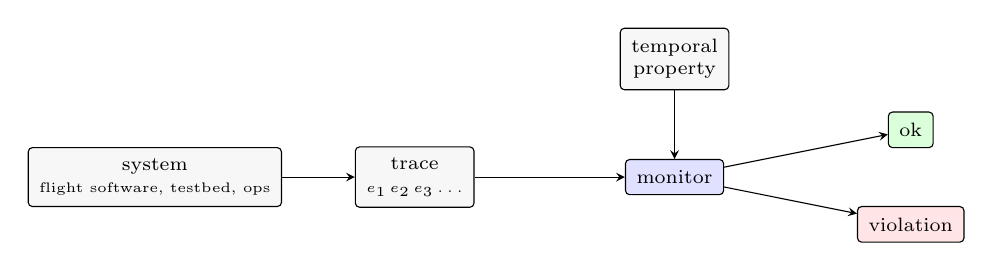
\begin{tikzpicture}[
  font=\scriptsize, >=stealth,
  b/.style={draw, rounded corners=1.5pt, align=center, inner sep=4pt, fill=black!3},
  lab/.style={font=\tiny, inner sep=1.5pt}
]
  \node[b] (sys) at (0,0)    {system\\{\tiny flight software, testbed, ops}};
  \node[b] (tr)  at (3.3,0)  {trace\\{\tiny $e_1\,e_2\,e_3\ldots$}};
  \node[b, fill=blue!12] (mon) at (6.6,0) {monitor};
  \node[b] (spec) at (6.6,1.5) {temporal\\property};
  \node[b, fill=green!14] (ok)  at (9.6,0.6)  {ok};
  \node[b, fill=red!10]   (bad) at (9.6,-0.6) {violation};

  \draw[->] (sys) -- (tr);
  \draw[->] (tr)  -- (mon);
  \draw[->] (spec) -- (mon);
  \draw[->] (mon) -- (ok);
  \draw[->] (mon) -- (bad);
\end{tikzpicture}\par}

\pause
\vspace{0.35cm}

No model to build and justify, and it scales to any system that can be made to
talk. The price: it says nothing about the runs you did not observe.

\end{frame}

%----------------------------------------
\begin{frame}[fragile]
  \frametitle{Writing monitors} \small

A monitor is an {\bf internal DSL} --- ordinary code in a host language, which
supplies the data handling for free. {\em Every dispatched command must eventually
succeed}, in \pycontract{}:

\begin{lstlisting}[language=python]
class Commands(Monitor):
    @initial
    class Start(AlwaysState):
        def transition(self, event):
            match event:
                case Dispatch(cmd, nr): return self.DoSucceed(cmd, nr)

    @data
    class DoSucceed(HotState):          # an obligation, not yet met
        cmd: str
        nr: int
        def transition(self, event):
            match event:
                case Succeed(self.cmd, self.nr): return ok
                case Fail(_, self.nr):  return error(f'{self.cmd} failed')
\end{lstlisting}

\pause

\ipromela{HotState} is the point: an obligation still {\em open} when the trace ends
is itself a violation. That is $\Box(p \rightarrow \Diamond q)$ with $nr$ bound ---
and the pattern matching is Python's, not ours.

\end{frame}

%----------------------------------------
\begin{frame}[fragile]
  \frametitle{\dejavu{}: an external DSL} \small

\dejavu{} goes the other way --- {\bf its own language}, not a host's. The same
obligation, turned into the past: {\em every command that succeeds was dispatched}.

\[
\forall c.\,\forall n.\ \mathit{succeed}(c,n) \rightarrow\;
\DDiamond\, \mathit{dispatch}(c,n)
\]

Fifteen lines of Python become one line of {\bf first-order past LTL} --- no state
machine, no bookkeeping of which pairs are outstanding. The quantifiers do it.

\pause
\vspace{0.3cm}

\begin{block}{}\small
\centering
Under the hood, {\bf BDDs} store the data --- which is what makes the monitoring
efficient.
\end{block}

\end{frame}

%----------------------------------------
\begin{frame}
  \frametitle{Five tools, and where they were used} \small

\begin{center}\scriptsize
\renewcommand{\arraystretch}{1.35}
\setlength{\tabcolsep}{4pt}
\begin{tabular}{|l|l|>{\raggedright\arraybackslash}p{2.35cm}%
                    |>{\raggedright\arraybackslash}p{2.1cm}%
                    |>{\raggedright\arraybackslash}p{2.1cm}|}
\hline
\rowcolor{blue!10}
& {\bf Host} & {\bf Formalism} & {\bf Engine} & {\bf Applied in}\\
\hline
\ours{\tc{}}         & Scala  & LTL + state machines    & formula rewriting       & \ladee{}\\
\hline
\ours{\logfire{}}    & Scala  & rules, facts in and out & Rete                    & \msl{}\\
\hline
\ours{\daut{}}       & Scala  & data automata           & indexed state machines  & \msnEndurance{}\\
\hline
\ours{\pycontract{}} & Python & data automata           & indexed state machines  & \msnEndurance{}
                                                                             \clipper{}\\
\hline
\ours{\dejavu{}}     & ---    & first-order past LTL    & BDDs over data          & ---\\
\hline
\end{tabular}
\end{center}


\end{frame}
